\documentclass[conference]{IEEEtran}
\IEEEoverridecommandlockouts
% The preceding line is only needed to identify funding in the first footnote. If that is unneeded, please comment it out.
\usepackage{cite}
\usepackage{amsmath,amssymb,amsfonts}
\usepackage{algorithmic}
\usepackage{graphicx}
\usepackage{textcomp}
\usepackage{xcolor}
\usepackage[caption=false, font=footnotesize]{subfig}
\def\BibTeX{{\rm B\kern-.05em{\sc i\kern-.025em b}\kern-.08em
    T\kern-.1667em\lower.7ex\hbox{E}\kern-.125emX}}
\begin{document}

\title{Estimating Subgraph Generation Models}

\author{\IEEEauthorblockN{1\textsuperscript{st} Laurens Bogaardt}
\IEEEauthorblockA{\textit{Netherlands eScience Center} \\
Amsterdam, the Netherlands \\
l.bogaardt@esciencecenter.nl}
\and
\IEEEauthorblockN{2\textsuperscript{nd} Frank Takes}
\IEEEauthorblockA{\textit{University of Amsterdam}\\
Amsterdam, the Netherlands\\
takes@uva.nl}
}

\maketitle

\begin{abstract}
Recently, a new network formation model was proposed. The current research looks into a method to estimate the parameters of this model based on the subgraph census.
\end{abstract}

\begin{IEEEkeywords}
Networks, Graphs, ERGM, SUGM, Subgraphs
\end{IEEEkeywords}

\section{Introduction}

The Exponential Random Graph Model (ERGM) is the most frequently used network formation model. However, it suffers from two fundamental flaws~\cite{Chandrasekhar2014}. Firstly, its parameter estimates are inconsistent. Secondly, it does not scale well. Recently, an alternative network formation model was suggested: the Subgraph Generation Model (SUGM)~\cite{Chandrasekhar2014}.

The original article describing SUGM contains two methods to estimate the parameters of the model. The current research suggests a third, more intuitive method based on the subgraph census. In an $k$-subgraph census, a network of $n$ nodes is partitioned into all possible subsets of $k$ nodes, which are then tallied according to their isomorphism class~\cite{Davis1972}.

\section{Subgraph Generation Model}

A SUGM is defined by a set of $l$ small subgraphs, such as links, triangles or stars, each with corresponding probabilities. For each subgraph $i$ of $m_{i}$ nodes, the $n$ nodes of the entire network are partitioned into all possible subsets of $m_{i}$ nodes. Then, each of these subsets receives the subgraph $i$ with propability $1-p_{i}$ or remains empty with probability $p_{i}$.

The observed network (left in Fig.~\ref{fig:Figure02}) is the union of all these subgraphs (right in Fig.~\ref{fig:Figure02}), where the generated subgraphs may overlap. Multiple neighbouring subgraphs may incidentally form additional structures such as triangles or squares.

\begin{table}[h!]
\def\arraystretch{1.6}
\caption{Probabilities in the Subgraph Census}
\begin{center}
\begin{tabular}{|c|c|c|c|c|}
\hline
\textbf{}&\multicolumn{4}{|c|}{\textbf{Subgraphs of the Undirected Triad Census}} \\
\cline{2-5}
\textbf{Model}&\includegraphics[scale=0.8]{Figure03_1.pdf}&\includegraphics[scale=.8]{Figure03_2.pdf}&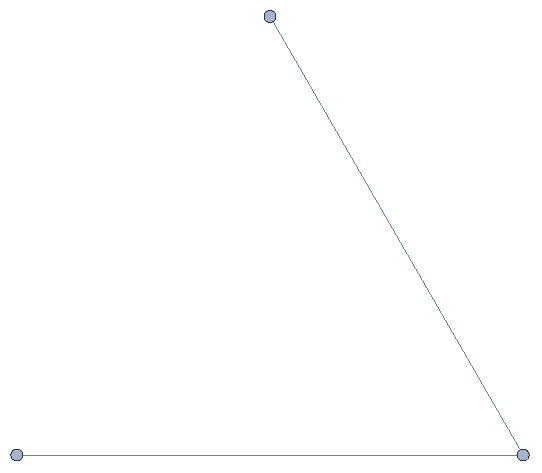
\includegraphics[scale=.8]{Figure03_3.pdf}&\includegraphics[scale=.8]{Figure03_4.pdf}\\
\hline
Links & $p_{L}^{3}$ & $3 \, p_{L}^{2} \, (1-p_{L})$ & $3 \, p_{L} \, (1-p_{L})^{2}$ & $(1-p_{L})^{3}$ \\
\hline
Triangles & $p_{T} \, (p_{T}^{n - 3})^{3}$ & $3 \, p_{T} \, (p_{T}^{n - 3})^{2} \, (1 - p_{T}^{n - 3})$ & $3 \, p_{T} \, (p_{T}^{n - 3}) \, (1-p_{T}^{n - 3})^{2}$ & $(1 - p_{T}) + p_{T} \, (1 - p_{T}^{n - 3})^{3}$ \\
\hline
Links \& Triangles & $p_{T} \, (p_{L} \, p_{T}^{n - 3})^{3}$ & $3 \, p_{T} \, (p_{L} \, p_{T}^{n - 3})^{2} \, (1 - p_{L} \, p_{T}^{n - 3})$ & $3 \, p_{T} \, (p_{L} \, p_{T}^{n - 3}) \, (1 - p_{L} \, p_{T}^{n - 3})^{2}$ & $(1 - p_{T}) + p_{T} \, (1 - p_{L} \, p_{T}^{n - 3})^{3}$ \\
\hline
\end{tabular}
\label{tab:Table1}
\end{center}
\end{table}

\begin{figure}[htbp]
\begin{center}
\captionsetup[subfigure]{width=40mm}
\subfloat{\label{fig:Figure02_1.pdf}\includegraphics[scale=.35]{Figure02_1.pdf}}
\hfill
\subfloat{\label{fig:Figure02_1.pdf}\includegraphics[scale=.35]{Figure02_2.pdf}}
\caption{The observed network (left) is the union (right) of randomly generated links (red), 2-paths (purple), triangles (green) and 3-stars (yellow).}
\vspace{-5mm}
\label{fig:Figure02}
\end{center}
\end{figure}

Table~\ref{tab:Table1} contains the probabilities of observing any of the possible triads for three different generation models. These probabilities $f_{j}$ enter into the multinomial probability mass function of~\eqref{eq:Multinomial}, together with the counts $x_{j}$ of the census, to form the likelihood function. This can be used to estimate the parameters of the model and their confidence intervals.
\begin{equation}
\mathcal{L}(f_{1}, \cdots, f_{l} | x_{1}, \cdots, x_{l}) = \frac{\Gamma(\sum_{j} x_{j}+1)}{\prod_{j} \Gamma(x_{j}+1)} \prod_{j=1}^{l} f_{j}^{x_{j}}
\label{eq:Multinomial}
\end{equation}

\section{Further Research}

Future work should extend the list of possible subgraphs, deal with the correlations within the census, develop an \mbox{\textit{R}-package} and apply the model to real-world data.

\bibliographystyle{IEEEtran}
\bibliography{Bibliography}

\end{document}
